\section{Discussion}\label{sec:discussion}
The transformation between genotype and phenotype is quite straight forward in
this project. The transformation is direct where some number of sequential bits in the bit
array determines the value in the phenotype. The genotype is fixed length which
makes the conversion quite easy. The only problem which could arise is the
problem of mutation in regular binary to integer conversion. For this project
that challenge was solved using Gray coding, as described above, which to some
extent solves the problem. This step does however introduce a small step between
binary and integer, but it would still be classified as direct. Since the
conversion is between binary and integers the underlying model would be
data oriented as compared to program oriented.

\subsection{Practical Implications}\label{sec:practical-implications}
The practical implications of this project is very interesting as it actually
can be used to do some real simulation and not just trivial problems. The
current implementation might not be robust enough to be published, but with some
more work it could actually be used.

For use in the real world, this tool could be used to match up spike trains from
the brain to test out either new models or trying to find the proper
configuration in already tried model, very much like the 12 cases tested
previously. One example which I can think of off the top of my head, is the use
in brain computer interfaces(BCI). In BCI one want to match up spike trains to
certain thoughts in the brain, this problem is of course a
regression/classification problem, but testing the models of what a person could
be thinking could be tested with this tool and even developing the model to
optimize the classification algorithm could use this tool.

A computational neuroscientist could of course also use this tool in the same
way we have used it, trying to match a model of spiking neurons to actual
spiking neurons. From my understanding of what they would do they could use this
tool to model neurons trying to approximate real spike trains and use those
models further to try and understand the underlying processes in the brain, but
also have a way of testing how one neuron or a group of neurons impact their
neighbours.

\subsection{Other Uses}\label{sec:other-uses}
There are several other uses for a more general version of this tool. Any place
where there are some results and a model trying to explain those results a
similar tool to this project could be used. For instance in complex mathematics
or physics we could have a result from the real world and trying to come up with
a model explaining it. If that model contains several variables which can be
mapped in the same fashion as in this project we can often use EA to solve the
problem. Often times such a complex model
might also be to big to efficiently approach with other methods, but with an EA
we can get close enough very fast. Another domain is in financial analysis where
the complexities of the system is to big to model in real time, but we would
still like to know what is going on. For such a problem we could, after the
fact, try and do model fitting and try to explain anomalies or maybe explain in
a bit more detail why the curve is the way it is to try and help.

To extend on the example of financial analysis we can think about events like
\href{http://en.wikipedia.org/wiki/Flash_crash}{Flash crash} which for a long
time remained a mystery. The reason was ultimately a combination of several
factors, but key among them was automatic traders. These events are extremely
hard to predict beforehand and are also very hard to analyse after the fact.
This tool could potentially help to analyse such event by helping to verify
models. To an extent this tool could also be used to try and understand
electronic traders which are often company secrets and very hard to predict.
With knowledge about automatic traders and how they act the large stock exchanges could help
prevent events such as the one linked to above. In figure \ref{fig:ea-financial}
there is a rudimentary illustration of the above example.

\begin{figure}
	\centering
	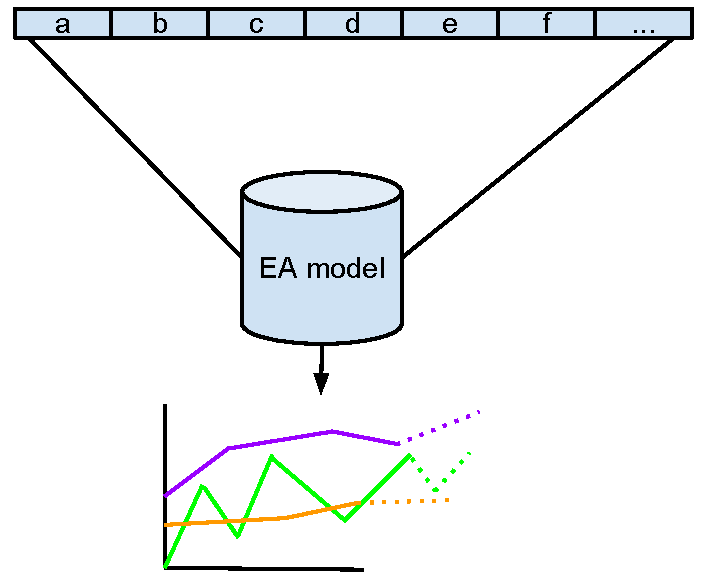
\includegraphics{ea-model.pdf}
	\caption{An illustration of financial analysis using Evolutionary
	algorithms}
	\label{fig:ea-financial}
\end{figure}
